\documentclass{article}

\usepackage{graphicx}
\usepackage{amsmath}

\usepackage[margin=1.5in]{geometry}

\title{Predicting Income Levels through the ID3 Decision Tree Algorithm}
\author{Ayla Lampard, Jason Uanon}

\begin{document}
\maketitle

\begin{figure*}
    \centering
    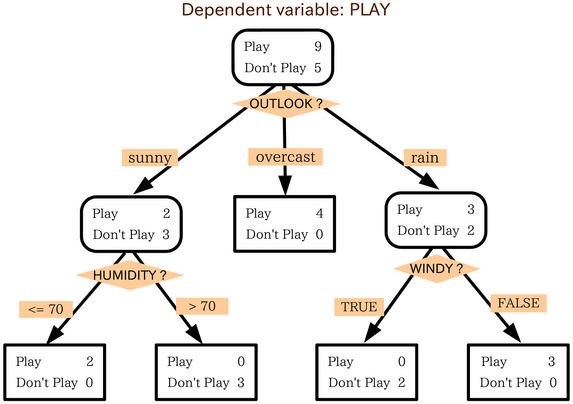
\includegraphics[width=\textwidth]{figs/decision_tree.png}
    \caption{Example of a decision tree}
    \label{decision_tree}
\end{figure*}

\section{Introduction}



\subsection{Motivation}

\textbf{Machine learning} is a branch of artificial intelligence that creates systems (computer programs) capable of autonomously learning and improving from data. Such systems are supplied with a set of "training data" that is then used to make predictions or generalizations about future instances. Statistics and information theory is used in machine learning to help assist systems in making the best possible "guess."

One approach to machine learning is the use of a \textbf{decision tree} algorithm. Decision tree systems use a tree-like graph (a decision tree) to model decisions in machine learning. At each node of the tree a decision can be made that narrows down the possibilities, eventually reaching a "leaf node" that contains that tree's prediction. Figure~\ref{decision_tree} shows an example of a decision tree.

Decision trees provide a simple model for us to answer general questions of the form: given training data that contains attributes $X = \{x_1, \ldots, x_n\}$ and satisfying a trait $y$, can we predict whether future instances of this data also satisfy $y$?


\subsection{Data}
We will be using the Adult Data Set from the UCI Machine Learning Repository \cite{bache-lichman}. This data is freely-available online and comes from the 1994 U.S. Census. It contains over 32,000 training instances and 16,000 test instances (although it does contain missing values, denoted with "?"). 

Using this data, we will create a decision tree that will predict whether a person's income exceeds \$50,000 per year. The data itself contains 14 attributes, which are (listed with their data categories):

\begin{itemize}
\item age: continuous. 
\item workclass: Private, Self-emp-not-inc, Self-emp-inc, Federal-gov, Local-gov, State-gov, Without-pay, Never-worked. 
\item fnlwgt: continuous. 
\item education: Preschool, 1st-4th, 5th-6th, 7th-8th, 9th, 10th, 11th, 12th,  HS-grad, Some-college, Assoc-voc, Assoc-acdm, Prof-school, Bachelors, Masters, Doctorate. 
\item education-num: continuous. 
\item marital-status: Married-civ-spouse, Divorced, Never-married, Separated, Widowed, Married-spouse-absent, Married-AF-spouse. 
\item occupation: Tech-support, Craft-repair, Other-service, Sales, Exec-managerial, Prof-specialty, Handlers-cleaners, Machine-op-inspct, Adm-clerical, Farming-fishing, Transport-moving, Priv-house-serv, Protective-serv, Armed-Forces. 
\item relationship: Wife, Own-child, Husband, Not-in-family, Other-relative, Unmarried. 
\item race: White, Asian-Pac-Islander, Amer-Indian-Eskimo, Other, Black. 
\item sex: Female, Male. 
\item capital-gain: continuous. 
\item capital-loss: continuous. 
\item hours-per-week: continuous. 
\item native-country: United-States, Cambodia, England, Puerto-Rico, Canada, Germany, Outlying-US(Guam-USVI-etc), India, Japan, Greece, South, China, Cuba, Iran, Honduras, Philippines, Italy, Poland, Jamaica, Vietnam, Mexico, Portugal, Ireland, France, Dominican-Republic, Laos, Ecuador, Taiwan, Haiti, Columbia, Hungary, Guatemala, Nicaragua, Scotland, Thailand, Yugoslavia, El-Salvador, Trinadad \& Tobago, Peru, Hong, Holand-Netherlands.
\end{itemize}

The initial tree will be created using the training data; the tree will then be tested on the test data, giving us feedback on its accuracy.

\section{Problem Setup}

\subsection{Definitions}

We will first define some terms that will be used. Note that the following formulas use the logarithm with base $2$. The natural logarithm (with base $e$) is often used, but in this case, information theory deals with bits of information: 0 or 1. Hence, the formulas describe the amount of "disorder" that can be expected among the bits used.

\textbf{Entropy} $H(X)$ measures the amount of disorder (or uncertainty) in a random variable \cite{segaran2007}. Let $X$ be a random variable from our data set with events ${x_1, x_2,...,x_n}$ and let $p(x_i)$ be the proportion of the elements $X = x_i$.  Mathematically the entropy of $X$ can be expressed  
\begin{align*}
 H(X) &= \sum_{i=1}^{n} p(x_i)\log_{2}\left(\frac{1}{p(x_i)}\right) \\
&= -\sum_{i=1}^{n}p(x_i)\log_{2}\left(p(x_i)\right)
\end{align*}

The \textbf{conditional entropy} of a random variable $X$ with events ${x_1,..,x_m}$ conditioned on another random variable $Y$ with events ${y_1,...,y_n}$ is the entropy of $X$ given that $Y$ has taken on a certain value $Y=y_j$. We can express the entropy of X conditioned on Y as
$$ H(X|Y) = -\sum_{i=1}^{n}p(x_i)\sum_{j=1}^{m}p(y_j|x_i)\log_2\left(p(y_j|x_i)\right) $$

The \textbf{information gain} of a random variable $X$ conditioned on a random variable $Y$ is

$$ IG(X) = H(Y) - H(Y|X) $$

Information gain will be our primary criterium that will determine what attribute to next split on; it is used in the ID3 decision tree algorithm to find the best attribute (e.g., the one that probabilistically reveals the most information regarding our target classification) \cite{mitchell1997}.

Another way to interpret information gain is the expected reduction in entropy (disorder) caused by partitioning the examples according to this attribute.

\subsection{The Algorithm}

We will be using the ID3 Decision Tree algorithm using information gain as the splitting criteria. It can be summarized as follows:

\begin{itemize}
\item Start from the empty decision tree
\item Select the next best attribute $i$ that maximizes information gain (i.e., maximizing $IG(X_i)$)
\item Recursively build the children of the root node
\end{itemize}

It is essentially a greedy algorithm that grows the tree top-down, continuing until the tree either classifies all of the training examples, or until all attributes have been used (for our purposes, with thousands of training examples, the latter case will most likely occur).\\

\subsection{Overfitting \& Pruning}

The algorithm previously described grows each branch of the tree just enough to perfectly classify the training examples. When the number of training examples is too small to produce a representative sample of the true target funtion (i.e., how the data behaves asymptotically), this can lead to suboptimal behavior on the test data \cite{mitchell1997}. There may also be ``noise" in the data that misrepresents the target function. In these cases, we may produce trees that overfit the data. More precisely, given a hypothesis space $H$, a hypothesis $h \in H$ is said to \textbf{overfit} the training data if there exists some alternative hypothesis $h' \in H$ such that $h$ has a smaller error rate than $h'$ over the training data, but $h'$ has a smaller error rate than $h$ over the entire distribution of instances \cite{mitchell1997}. 

One heuristic to reduce overfitting is to \textbf{prune} the tree. That is, we seek to reduce the size of the decision tree while minimizing the effect on the training set. We could cross check with the test data or a validation set to check if pruning actually increases accuracy on the overall data set.

\subsection{Implementation}

We will be using Python 2.7.3 for the implementation of the decision tree algorithms. As part of the project, we will also create a Cython version using Cython 0.15.1 to enhance its performance, and compare the relative speeds of the two implementations.\\

For more information on our implementation see our code in \verb+/src/predictor+.


\section{Results}

\subsection{Data}
Results of decision tree algorithm on test data prior to Cythonization:\\
$\begin{array}{ll}
$Correct:$& 13195/16281 (81.05\% $ accuracy$)\\
$Incorrect:$& 3086/16281\\
$Average run time:$ & 54$ seconds$
\end{array}$\\

Results of decision tree algorithm on test data after Cythonization:\\
$\begin{array}{ll}
$Correct:$& 13195/16281 (81.05\% $ accuracy$)\\
$Incorrect:$& 3086/16281\\
$Average run time:$ & 36$ seconds$
\end{array}$\\

\subsection{Interpretation}
After Cythonizing the decision\_tree module (that does the decision tree calculations) alone, there was a big speed boost from simply compiling the functions. We left the file reading portions in pure Python, which is probably the biggest bottleneck within the whole program. But we left it in there since we used quite a bit of Python's dynamic arrays for convenience, and it would involve a non-trivial change to convert it into c-style arrays (with manual memory management, etc.).

\subsection{Possible improvements}
\textbf{Pruning:} This tree was fully built (i.e., each branch was extended until it ran out of attributes or examples to classify) from the training data (with 32,561 examples) and has most likely been over-fit. \\

\textbf{Validation:} Along the same lines, we could have split off some of the training set into a validation set, which could have been used with pruning. \\ 

\textbf{Attribute values:} Some of the attributes had continuous instead of categorical data, and examples were converted heuristically into categories. The selections could have been improved on a case-by-case basis, e.g., a 5 year difference could make a big difference for younger people, but not so much for older people.\\

\textbf{Missing values:} Some of the data (training and test) had missing values. For the training data, this could have skewed some of the probabilities slightly. For test data, if it was missing a value we simply picked the leftmost child and continued. Instead we could have made a more reasonable choice, e.g., choose the child corresponding to the value that is most likely given the training data.\\

\textbf{Better Cython implementation:} There is room to dig deeper into Cython and find more things to optimize. For instance, we could use C functions for file i/o and example processing.


\begin{thebibliography}{9}

\bibitem{bache-lichman}
Bache, K. and Lichman, M. (2013). \textsl{UCI Machine Learning Repository: Adult Data Set}. [http://archive.ics.uci.edu/ml/datasets/Adult]. Irvine, CA: University of California, School of Information and Computer Science.

\bibitem{segaran2007}
Segaran, Toby. \textsl{Programming Collective Intelligence}. O'Reilly, California, 2007.

\bibitem{mitchell1997}
Mitchell, Tom. \textsl{Machine Learning}. McGaw-Hill, 1997.

\end{thebibliography}

\end{document}
